\documentclass[12pt,utf8,notheorems]{beamer}

\usepackage[ngerman]{babel}

\usepackage{amsmath,amssymb}
%\usepackage[framed,amsmath,thmmarks,hyperref]{ntheorem}

%\usepackage[small,nohug]{diagrams}
%\diagramstyle[labelstyle=\scriptstyle]

%\usepackage[protrusion=true,expansion=false]{microtype}

%\usepackage{lmodern}
\usepackage{nicefrac}
\usepackage{tabto}
\usepackage{tikz}
\usetikzlibrary{decorations.pathreplacing}
\usepackage{bussproofs}
\usepackage{stmaryrd}

%\usepackage[natbib=true,style=numeric]{biblatex}
%\usepackage[babel]{csquotes}
%\bibliography{lit}

%\usepackage{hyperref}

\setlength\parskip{\medskipamount}
\setlength\parindent{0pt}

%\theoremseparator{:}
\theoremstyle{plain}  %nonumberplain
%\newtheorem{beh}{Behauptung}
\newtheorem{proposition}{Proposition}
\newtheorem{corollary}{Korollar}
\newtheorem{theorem}{Satz}
\theoremstyle{definition}
\newtheorem{definition}{Definition}
%\newtheorem{kor}{Korollar}
%\newtheorem{satz}{Satz}
%\newtheorem{lemma}{Lemma}
%\newtheorem{hilfsaussage}{Hilfsaussage}
%\theorembodyfont{\normalfont}
\newtheorem{axiom}{Axiom}
%\newtheorem{defnprop}{Definition/Proposition}
%\newtheorem{bem}{Bemerkung}
%\newtheorem{bsp}{Beispiel}
%\theoremsymbol{\ensuremath{\openbox}}
%\newtheorem{proof}{Beweis}
%\newtheorem{defn}{Definition}

\newcommand{\lra}{\longrightarrow}
\newcommand{\lhra}{\ensuremath{\lhook\joinrel\relbar\joinrel\rightarrow}}
\newcommand{\thlra}{\relbar\joinrel\twoheadrightarrow}

\newcommand{\Z}{\mathbb{Z}}
\renewcommand{\C}{\mathbb{C}}
\newcommand{\N}{\mathbb{N}}
\newcommand{\Hom}{\mathrm{Hom}}
\newcommand{\Spur}[1]{\operatorname{Spur}#1}
\newcommand{\SpurDyn}[1]{\operatorname{Spur}\left(#1\right)}
\newcommand{\rank}[1]{\operatorname{rank}#1}
\newcommand{\Ker}[1]{\operatorname{ker}#1}
\newcommand{\Bild}[1]{\operatorname{im}#1}
\newcommand{\sgn}[1]{\operatorname{sgn}#1}
\newcommand{\id}{\mathrm{id}}
\newcommand{\Aut}[1]{\operatorname{Aut}(#1)}
\newcommand{\GL}[1]{\operatorname{GL}(#1)}
\newcommand{\freist}{\_{}\_{}}

\renewcommand{\O}{\mathcal{O}}
\renewcommand{\P}{\mathcal{P}}
\newcommand{\1}{\mathbf{1}}
\renewcommand{\_}{\mathpunct{.}\,}
\newcommand{\?}{\,{:}\,}
\newcommand{\seq}[1]{\mathrel{\vdash\!\!\!_{#1}}}
\renewcommand{\ll}[1]{\llbracket{#1}\rrbracket}

\newcommand{\XXX}[1]{\textcolor{red}{#1}}

%\newarrow{Equals}=====

\title{Konstruktive Mathematik}
\author{Ingo Blechschmidt \\ mit Illustrationen von Carina Willbold}
%\subtitle{Vektorbündel, K-Theorie und \\ charakteristische Klassen}
%\institute{Sommerakademie in Neubeuern}
%\date{7. August 2012}

%\usetheme{Warsaw}  %Warsaw, Berkeley?
\usetheme{Warsaw}
\useoutertheme{split}
\usecolortheme{seahorse}
\usefonttheme{serif}
\usepackage{palatino}
\useinnertheme{rectangles}
%\usepackage{bookman}
%\setbeamercovered{transparent}

\setbeamertemplate{navigation symbols}{}
\setbeamertemplate{footline}{}
\setbeamertemplate{headline}{}

\beamertemplateboldcenterframetitle
%\setbeamerfont{frametitle}{size={\Large}}

\newenvironment{changemargin}[2]{%
  \begin{list}{}{%
    \setlength{\topsep}{0pt}%
    \setlength{\leftmargin}{#1}%
    \setlength{\rightmargin}{#2}%
    \setlength{\listparindent}{\parindent}%
    \setlength{\itemindent}{\parindent}%
    \setlength{\parsep}{\parskip}%
  }%
  \item[]}{\end{list}}

\begin{document}

\setbeameroption{show notes}
\setbeamertemplate{note page}[plain]

\frame[plain]{
  \begin{center}
    
\includegraphics[scale=0.65]{fortune-teller.png}
  \end{center}
}

\frame[t]{\frametitle{Informale Bedeutung logischer Formeln}
  \tikz[remember picture] \node[coordinate,yshift=0.0em] (n0) {};
  \vspace{-1.5em}
  \begin{description}\small
    \item[$\bot$] Es stimmt eine Falschheit.
    \tikz[remember picture] \node[coordinate,yshift=0.5em] (n2) {};
    \item[$A \wedge B$] $A$ und $B$ stimmen.
    \item[$A \vee B$] $A$ oder $B$ stimmt.
    \item[$A \Rightarrow B$] Sollte~$A$ stimmen, dann auch~$B$.
    \item[$\forall x{\in}X\_\! A(x)$] Für alle~$x \in X$ stimmt jeweils~$A(x).$
    \item[$\exists x{\in}X\_\! A(x)$] Es gibt mindestens ein~$x \in X$, für das~$A(x)$
    stimmt.
    \tikz[remember picture] \node[coordinate,yshift=-0.0em] (n1) {};
  \end{description}
  \vspace{1em}

  \begin{description}\small
    \item[$\bot$] 
    \tikz[remember picture] \node[coordinate,yshift=0.5em] (n5) {};%
    Wir haben Beleg für eine Falschheit.
    \item[$A \wedge B$] Wir haben Beleg für~$A$ und für~$B$.
    \item[$A \vee B$] Wir haben Beleg für~$A$ oder für~$B$.
    \item[$A \Rightarrow B$] Sollten wir Beleg für~$A$ haben, können wir
    (gleichmäßig) auch Beleg für~$B$ konstruieren.
    \item[$\forall x{\in}X\_\! A(x)$] Wir können (gleichmäßig) für alle~$x \in X$
    Belege für~$A(x)$ konstruieren.
    \item[$\exists x{\in}X\_\! A(x)$] Wir haben ein~$x \in X$ zusammen mit Beleg
    für~$A(x)$.
    \tikz[remember picture] \node[coordinate,yshift=-0.0em] (n4) {};
  \end{description}

  \begin{tikzpicture}[overlay,remember picture]
    \path (n2) -| node[coordinate] (n3) {} (n0);
    \path (n1) -| node[coordinate] (n33) {} (n0);
    \draw[thick,decorate,decoration={brace,amplitude=5pt}]
            (n33) -- (n3) node[midway,left=4pt] {kl.};
    \path (n5) -| node[coordinate] (n6) {} (n0);
    \path (n4) -| node[coordinate] (n44) {} (n0);
    \draw[thick,decorate,decoration={brace,amplitude=5pt}]
            (n44) -- (n6) node[midway,left=4pt] {int.};
  \end{tikzpicture}

  \begin{tikzpicture}[remember picture,overlay]  
    \node [xshift=-1cm,yshift=-5.5cm] at (current page.north east)
      {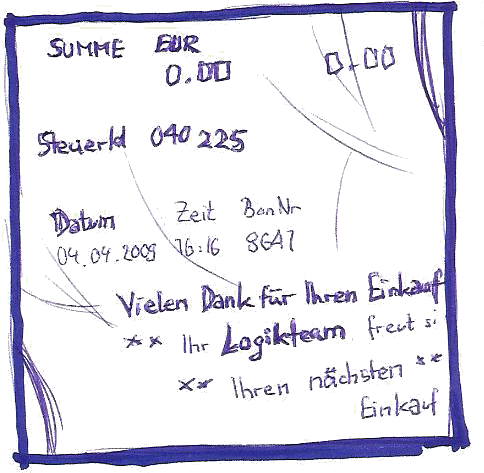
\includegraphics[scale=0.3]{evidence.png}};
  \end{tikzpicture}
}

\frame[t]{%\frametitle{Gentzens Kalkül natürlichen Schließens}
  \small
  \begin{itemize}
    \item Strukturelle Regeln: \\
    \vspace{-1em}
    \phantom{a}\hfill
    \AxiomC{$\phantom{\seq{\vec x}}$}\UnaryInfC{$A \seq{\vec x} A$}\DisplayProof\hfill
    \AxiomC{$A \seq{\vec x} B$}\UnaryInfC{$A[\vec s/\vec x]
    \seq{\vec y} B[\vec s/\vec x]$}\DisplayProof\hfill
    \AxiomC{$A \seq{\vec x} B$}\AxiomC{$B \seq{\vec x}
    C$}\BinaryInfC{$A \seq{\vec x} C$}\DisplayProof\hfill
    \phantom{a}
    \vfill
    \item Regeln für Konjunktion: \\
    \AxiomC{$\phantom{\seq{\vec x}}$}\UnaryInfC{$A \seq{\vec x} \top$}\DisplayProof\hfill
    \AxiomC{$\phantom{\seq{\vec x}}$}\UnaryInfC{$A \wedge B \seq{\vec x} A$}\DisplayProof\hfill
    \AxiomC{$\phantom{\seq{\vec x}}$}\UnaryInfC{$A \wedge B \seq{\vec x} B$}\DisplayProof\hfill
    \AxiomC{$A \seq{\vec x} B$}\AxiomC{$A \seq{\vec x} C$}\BinaryInfC{$A \seq{\vec x} B \wedge C$}\DisplayProof
    \vfill
    \item Regeln für Disjunktion: \\
    \AxiomC{$\phantom{\seq{\vec x}}$}\UnaryInfC{$\bot \seq{\vec x} A$}\DisplayProof\hfill
    \AxiomC{$\phantom{\seq{\vec x}}$}\UnaryInfC{$A \seq{\vec x} A \vee B$}\DisplayProof\hfill
    \AxiomC{$\phantom{\seq{\vec x}}$}\UnaryInfC{$B \seq{\vec x} A \vee B$}\DisplayProof\hfill
    \AxiomC{$A \seq{\vec x} C$}\AxiomC{$B \seq{\vec x} C$}\BinaryInfC{$A \vee B \seq{\vec x} C$}\DisplayProof
    \vfill
    \item Doppelregel für Implikation: \\
    {\centering \AxiomC{$A \wedge B \seq{\vec x} C$}\doubleLine\UnaryInfC{$A \seq{\vec x} B \Rightarrow C$}\DisplayProof\par}
    \vfill
    \item Doppelregeln für Quantifikation: \\
    \vspace{-0.7em}
    \phantom{a}\hfill
    \AxiomC{$A \seq{\vec x, y} B$}\doubleLine\UnaryInfC{$\exists y\_\! A \seq{\vec x} B$}\DisplayProof\hfill
    \AxiomC{$A \seq{\vec x, y} B$}\doubleLine\UnaryInfC{$A \seq{\vec x} \forall y\_\! B$}\DisplayProof\hfill
    \phantom{a}
  \end{itemize}
}

\end{document}
